\documentclass{amia}
\usepackage{graphicx}
\usepackage[labelfont=bf]{caption}
\usepackage[superscript,nomove]{cite}
\usepackage{color}


\begin{document}


\title{Chest X-Ray (CXR) Disease Diagnosis with DenseNet}

\author{Doug Beatty$^{1}$, Filip Juristovski$^{1}$, Rushi Desai$^{1}$, Mohamed Abdelrazik$^{1}$}

\institutes{
    $^1$Georgia Institute of Technology, Atlanta, Georgia\\
}

\maketitle

\noindent{\bf Abstract}

\textit{ Chest X-ray\cite{ref1} is a crucial medical imaging technology used by several doctors to diagnose patients. Training a human radiologist is a lengthy and costly process. Deep learning techniques combined with availability of larger data sets increases the feasibility of building automated models with  performance close to human radiologists. }

\textit{We present a scalable deep learning model trained on the CheXpert \cite{ref2} data set of X-ray images to detect and correctly classify 14 different diseases}

\section*{Introduction}
A chest radiograph\cite{ref1}, or a chest X-ray (CXR) is one of the oldest and most common forms of medical imaging. A human radiologist requires significant training time and cost to be able to perform a comprehensive chest X-ray analysis with minimal error. Several types of abnormalities can show up in a chest radiograph that can lead to detection and diagnosis of several kinds of diseases but due to the vast number of different abnormalities and the overlapping reasons that might cause them, there’s a plenty of room for human error.

The revolution of machine learning and deep learning techniques combined with the availability of larger data sets\cite{ref2} and big data processing systems\cite{ref3} makes the analysis of x-ray images increasingly more realistic and the creation of automated models more feasible. The objective of this project is to train an efficient and scalable deep learning model which can learn from a data set of X-ray images to detect and correctly classify 14 different diseases. Automating the X-ray analysis makes the overall diagnosing process faster and less error-prone which significantly improves the patient’s treatment procedure.




\section*{Approach}
\begin{enumerate}
\item Data set acquisition
\item Image preprocessing - Apache Spark
\item Training Dense 121 deep learning model - Keras
\item Model validation and fine tuning
\item Model evaluation
\end{enumerate}

\section*{Data acquisition }
Dataset was acquired upon registration and acceptance of the Stanford University School of Medicine CheXpert Dataset Research Use Agreement terms and conditions.\cite{ref2}

\section*{Dataset format}

Dataset consists of 224,316 chest radiographs of 65,240 patients. Each imaging study can pertain to one or more images, but most often are associated with two images: a frontal view and a lateral view. Images are provided with 14 labels derived from a natural language processing tool applied to the corresponding free-text radiology reports.

Image files are provided following a specific directory structure :

/[Data set type]/[patient ID]/[Study ID]/[View ID]\_[view type].jpg

where data set type can be train (for training set) or valid (for validation set), and view type can be frontal or lateral.

e.g. an input sample of a frontal study for a patient in the training set will be available at :

CheXpert/train/patient00001/study1/view1\_frontal.jpg

Each image is stored as a .jpg file with single channel (grey scale) where each pixel is stored as unsigned byte.

A CSV file is provided for each data set type (valid or train). Each image record contains a path, several medical labels for different diseases (such as Cardiomegaly, Edema, Pneumonia, and so on.), along with some demographic information about the patient such as sex and age.


\section*{Dataset Pre-Processing}

CheXpert\cite{ref2} images are provided in high resolution which is not suitable for use as input to the model. Using a high resolution image significantly increases the number of input feature vectors which would require an increase in the model complexity and training time. Data set images where prepossessed before training using Apache Spark which is a scalable Big data processing technology. Several down-sampling techniques were used to reduce image size.

A neural network (e.g. CNN) is said to have an in-variance property when it is capable to robustly classify objects even if its placed in different orientations.To enrich the input data set and increase the number of available training samples, we performed data augmentation by generating several images with different orientations from a subset of input images.

Each input image is down sampled by resizing to 224*224 pixels. An input image generates one or more augmented versions of itself (e.g. by horizontal flipping). Each output image is assigned an ID of type Long, and inherits all the labels from the original input image.

Preprocessed images are saved to HDFS, which is a highly distributed and scalable Big data storage system. Due to HDFS implementation and API limitations, storing several tiny image files is not an efficient operation.
We decided to change the output format of be textual. Each image can be represented with the unsigned values of its byte stream (a vector of length 224*224). Each Spark RDD Partition will save its images as a space separated file with this format:
[imageID] [bytes values]

Where Image ID is the newly assigned ID, and the bytes are space separated vector of row based pixel values.

A corresponding CSV file for labels is generated which starts with the Image Id along with all the inherited labels from the original image.

This new output storage format resulted in significant decrease of the preprocessing job run time, and was suitable as a direct input to the model.



\section*{Metrics}

This sentence has one reference citation\cite{ref1}.

This sentence has two reference citations\cite{ref1,ref2}.

More text of an additional paragraph, with a figure reference (Figure ~\ref{fig1}) and a figure inside a Word text box below.  Figures need to be placed as close to the corresponding text as possible and not extend beyond one page.\\
\begin{figure}[h!]
\centering
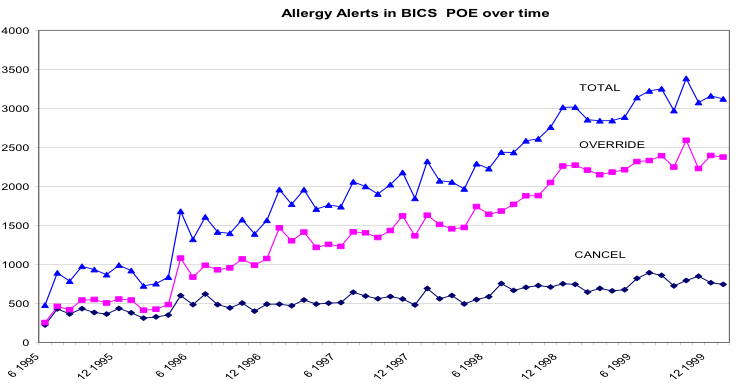
\includegraphics[scale=1]{pics/figure1.png}
\caption{Total allergy alerts, overridden alerts, or drug order cancelled.}
\label{fig1}
\end{figure}

This is additional text added just to show the one-column formatting.  This is additional text added just to show the one-column formatting.  This is additional text added just to show the one-column formatting.  This is additional text added just to show the one-column formatting.  This is additional text added just to show the one-column formatting.  This is additional text added just to show the one-column formatting.  This is additional text added just to show the one-column formatting.

This paragraph contains a reference to a table just below (Table 1).  All tables need to be placed as close to the corresponding text as possible, But each individual table should be on one page and not extend to multiple pages unless labeled as ``€œContinued"€.

\begin{table}[h]
\centering
\caption{Submission type, abstract length, and page length maximum for AMIA submissions.}
  \begin{tabular}{|l|l|l|}
  \hline
    \textbf{Submission Type}    & \textbf{Abstract Length}  & \textbf{Page Length Maximum**} \\ \hline
    Paper  & 125-150 words  & Ten   \\ \hline
    Student Paper  & 125-150 words  & Ten \\ \hline
    Poster  &50-75 words*   & One \\ \hline
    Podium  Abstract & 50-75 words*  & Two \\ \hline
    Panel   &150-200 words  & Three \\ \hline
    System Demonstrations    &150-200 words  & One \\ \hline
  \end{tabular}
\end{table}
*: All podium abstract and poster submissions must have a brief (50-75 words) abstract. The abstract does NOT have to be part of the document, but must be entered on the submission website in the Abstract box in Step 2.

**: \textcolor{red}{If your submission is longer than what is specified below, it will be rejected without review.}

This is another paragraph.

\section*{Experimental Results}
Experimental results are described here.

Lorem ipsum dolor sit amet, consectetur adipiscing elit. Nulla malesuada tempus lacus. Phasellus vestibulum ut dolor ut vestibulum. Sed tincidunt libero nibh. Donec nec accumsan felis. Etiam consectetur metus sit amet pellentesque fermentum. Morbi sagittis velit quis justo faucibus, quis mollis ipsum vestibulum. Phasellus condimentum quam id nisl fringilla fermentum. Curabitur vitae augue ornare, aliquet odio sit amet, faucibus metus. Maecenas finibus eget magna lacinia efficitur.


\section*{Discussion}
Discussion is here.

Vivamus bibendum pharetra varius. Vivamus viverra nisl sed ex fringilla, in rutrum mauris dignissim. Pellentesque malesuada mattis velit id bibendum. Nulla maximus, justo eu elementum blandit, urna turpis posuere sapien, vel facilisis tellus nunc sit amet turpis. Proin tincidunt rhoncus turpis, et rhoncus diam luctus ut. Sed id leo varius, vehicula augue quis, dictum ligula. Praesent eget ex nec arcu bibendum viverra id ut mi. Proin lobortis tempus tellus ut pretium. Aliquam pretium sapien eget urna venenatis tincidunt.

\section*{Conclusion}
Your conclusion goes at the end, followed by References, which must follow the Vancouver Style (see: www.icmje.org/index.html).  References begin below with a header that is centered.  Only the first word of an article title is capitalized in the References.

\section*{Rushi}
DenseNet are

\makeatletter
\renewcommand{\@biblabel}[1]{\hfill #1.}
\makeatother



\bibliographystyle{unsrt}
\begin{thebibliography}{1}
\setlength\itemsep{-0.1em}

\bibitem{ref1}
Siamak N. Nabili, M. (2019). Chest X-Ray Normal, Abnormal Views, and Interpretation. [online] eMedicineHealth.
\bibitem{ref2}
CheXpert: A Large Dataset of Chest X-Rays and Competition for Automated Chest X-Ray Interpretation. [Internet]. Stanfordmlgroup.github.io. 2019.
\bibitem{ref3}
FAN M, XU S. Massive medical image retrieval system based on Hadoop. Journal of Computer Applications. 2013;33(12):3345-3349.
\bibitem{ref4}
Huang G, Liu Z, van der Maaten L, Weinberger K. Densely Connected Convolutional Networks [Internet]. arXiv.org. 2019.
\bibitem{ref5}
Rajpurkar P, Irvin J, Zhu K, Yang B, Mehta H, Duan T et al. CheXNet: Radiologist-Level Pneumonia Detection on Chest X-Rays with Deep Learning [Internet]. arXiv.org. 2019.
\bibitem{ref6}
Liu H, Wang L, Nan Y, Jin F, Pu J. SDFN: Segmentation-based Deep Fusion Network for Thoracic Disease Classification in Chest X-ray Images [Internet]. arXiv.org. 2019.
\bibitem{ref7}
Wang X, Peng Y, Lu L, Lu Z, Bagheri M, Summers R. ChestX-Ray8: Hospital-Scale Chest X-Ray Database and Benchmarks on Weakly-Supervised Classification and Localization of Common Thorax Diseases. 2019.
\bibitem{ref8}
Yao L. Weakly supervised medical diagnosis and localization from multiple resolutions [Internet]. Arxiv.org. 2019.
\bibitem{ref9}
Guendel S, Grbic S, Georgescu B, Zhou K, Ritschl L, Meier A et al. Learning to recognize Abnormalities in Chest X-Rays with Location-Aware Dense Networks [Internet]. arXiv.org. 2019.
\bibitem{ref10}
Raoof S, Feigin D, Sung A, Raoof S, Irugulpati L, Rosenow E. Interpretation of Plain Chest Roentgenogram. 2019.
\bibitem{ref11}
Zhou B, Khosla A, Lapedriza A, Oliva A, Torralba A. Learning deep features for discriminative localization [Internet]. Arxiv.org. 2019.

\bibitem{ref 12}
http://www.stat.harvard.edu/Faculty\_Content/meng/JCGS01.pdf

\bibitem{ref98}
Pryor TA, Gardner RM, Clayton RD, Warner HR. The HELP system. J Med Sys. 1983;7:87-101.
\bibitem{ref99}
Gardner RM, Golubjatnikov OK, Laub RM, Jacobson JT, Evans RS. Computer-critiqued blood ordering using the HELP system. Comput Biomed Res 1990;23:514-28.




\end{thebibliography}

\end{document}
